\documentclass[11pt,aspectratio=169]{beamer}
\usetheme{Boadilla}
\usecolortheme{beaver}
\usepackage[utf8]{inputenc}
\usepackage{amsmath}
\usepackage{amsfonts}
\usepackage{amssymb}
\usepackage[spanish,mexico]{babel}
\usepackage{graphicx}
\usepackage{multicol}

% \usepackage{ucs}
% \usepackage{beamerthemeboxes}
% \usepackage{caption}
% \usepackage{mathpazo}
% \usepackage{fontenc}
% \usepackage{booktabs}
% \usepackage{listings}
% \usepackage{algorithm,algorithmic}

\date{\today}
\author{Dr. Héctor Selley}
\institute{Universidad Anáhuac México} 
\title[Introducción a la IA]{Introducción a la Inteligencia Artificial}


\begin{document}

% Título
\begin{frame}
    \titlepage
\end{frame}

% Índice
\begin{frame}
 \tableofcontents
\end{frame}

% ¿Qué es la IA?
\section{¿Qué es la IA?}
\begin{frame}{¿Qué es la IA?}
    \begin{block}{Inteligencia artificial}\pause
        La IA es un campo de estudio de las ciencias de 
        la computación que se ocupa de crear sistemas y programas capaces de 
        realizar tareas que normalmente requieren de la inteligencia humana. \pause
        El objetivo de la IA es desarrollar máquinas y sistemas que puedan 
        simular y emular la capacidad de percepción, razonamiento, aprendizaje 
        y toma de decisiones propias de los seres humanos.
    \end{block}
\end{frame}

\begin{frame}{¿Qué es la IA?}
    \begin{figure}
        \centering
        \includegraphics[scale=0.35]{"../Programacion para ML/Contenido/img/ML-multi.png"}
    \end{figure}
\end{frame}

\begin{frame}{¿Qué es la IA?}
    \begin{itemize}
        \item La inteligencia artificial se basa en algoritmos y modelos matemáticos 
            que permiten a las máquinas procesar grandes cantidades de datos, aprender 
            de ellos y tomar decisiones o realizar acciones en base a ese conocimiento. \pause
        \item En informática, la inteligencia expresada por máquinas, sus procesadores y 
            su software, que serían los análogos al cuerpo, el cerebro y la mente, 
            respectivamente, a diferencia de la inteligencia natural demostrada por humanos 
            y ciertos animales con cerebros complejos.\pause
	    \item En ciencias de la computación, una máquina \textit{inteligente} ideal es un 
            agente flexible que percibe su entorno y lleva a cabo acciones que maximicen 
            sus posibilidades de éxito en algún objetivo o tarea.\pause
        \item La inteligencia artificial no tiene como finalidad reemplazar a los humanos, 
            sino mejorar significativamente las capacidades y contribuciones de estos.  
    \end{itemize}
\end{frame}

\begin{frame}{¿Qué es la IA?}
    \begin{itemize}
        \item En 1956, John McCarthy acuñó\footnote{Acuñar: Dar forma a expresiones o 
            conceptos, especialmente cuando logran difusión o permanencia.} la expresión 
            \textit{inteligencia artificial}, y la definió como \textit{la ciencia e ingenio 
            de hacer máquinas inteligentes, especialmente programas de cómputo inteligentes}.
            \pause
        % \item La IA se divide en diferentes ramas, como el aprendizaje automático 
        %     (machine learning), el procesamiento del lenguaje natural, la visión artificial, 
        %     los sistemas expertos, entre otros.
        \item Se hizo presente poco después de la Segunda Guerra Mundial con el desarrollo 
            de la \textit{prueba de Turing}, mientras que la locución fue acuñada 
            por el informático John McCarthy en la Conferencia de Dartmouth. 
    \end{itemize}
\end{frame}

\begin{frame}{Prueba de Turing}
    \begin{multicols}{2}
    \begin{figure}
        \centering
        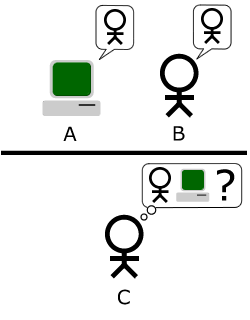
\includegraphics[scale=0.75]{img/Turing_Test_version_3.png}
    \end{figure}
    \begin{itemize}
        \item sacara
        \item asociadas
    \end{itemize}
\end{multicols}
\end{frame}

\begin{frame}{Prueba de Turing}
    \begin{figure}
        \centering
        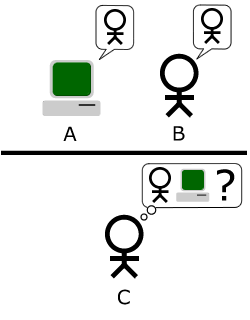
\includegraphics[scale=0.75]{img/Turing_Test_version_3.png}
    \end{figure}
    \begin{itemize}
        \item 
    \end{itemize}
\end{frame}

\begin{frame}{¿Qué es la IA?}
    John Searle introdujo una distinción entre los tipos de IA\pause \cite{searle}:
    \begin{itemize}
        \item IA fuerte \pause
        \item IA débil
    \end{itemize}
\end{frame}

\begin{frame}{¿Qué es la IA?}
    \begin{block}{IA fuerte}\pause
        La IA es la ciencia e ingeniería que permtirá replicar la inteligencia
        humana mediante máquinas.
    \end{block}\pause
    También conocida como \textbf{dura}, en ella se busca construir máquinas que
    razonen como lo hacen los humanos, este es el campo de trabajo de neurobiólogos
    y neurocientíficos, falta mucho por hacer.
\end{frame}

\begin{frame}{¿Qué es la IA?}
    \begin{block}{IA débil}\pause
        La IA es la ciencia e ingeniería que permite diseñar y programar
        ordenadores de forma que realicen tareas que requieren inteligencia.
    \end{block}\pause
    El objetivo no es reproducir exactamente los procesos de pensamiento humano,
    sino conseguir que las máquinas sean capaces de resolver problemas como lo 
    hacen las personas o inclusive mejor, en un dominio restringido.
\end{frame}

\begin{frame}{¿Qué es la IA?}

\end{frame}


% Historia
\section{Historia}
\begin{frame}{Historia}
    Historia
\end{frame}

\begin{frame}{Historia}
    \begin{figure}
        \centering
        \includegraphics[scale=0.35]{"../Programacion para ML/Contenido/img/AI-ML2.png"}
    \end{figure}
\end{frame}

% Aplicaciones
\section{¿Para qué sirve la IA?}
\begin{frame}{Aplicaciones}
    
\end{frame}

\section[Ética]{Dilemas éticos}
\begin{frame}{Privacidad}
    \begin{figure}
        \centering
        \includegraphics[scale=0.35]{"../Programacion para ML/Contenido/img/ads.jpg"}
    \end{figure}
\end{frame}

\begin{frame}{Privacidad}
    \begin{figure}
        \centering
        \includegraphics[scale=0.25]{"../Programacion para ML/Contenido/img/target.png"}
    \end{figure}
\end{frame}

\section*{Bibliografía}
\begin{frame}[allowframebreaks]{References}
    \nocite{*}
    \bibliographystyle{plain}
    \bibliography{biblioIA}
\end{frame}
\end{document}

